\section{Introduction and Research Questions}
\label{chapter:01}

% block-id: 01.introduction.heading
\hypertarget{01.introduction.heading}{}
\subsection{High-frequency loss and current sharing}

% block-id: 01.introduction.p1
\hypertarget{01.introduction.p1}{}
Litz wire controls high-frequency current through strand insulation and longitudinal transposition. Strand diameter sets the local skin-effect scale, neighboring conductors and the return shape proximity fields, and common terminals couple the complex strand currents. A structural comparison therefore requires both an electromagnetic model and consistent definitions of copper area, axial length, and terminal conditions.

% block-id: 01.introduction.p2
\hypertarget{01.introduction.p2}{}
Discrete-transposition modeling with two-dimensional FEM (DTM) \cite{P01} connects strand-position permutations to cross-sectional fields. Its extension to nonideal compound transposition (iDTM) \cite{N01} treats hierarchical and subbundle effects. Improved segmented equivalent circuits \cite{P02}, FEM–PEEC coupling \cite{P03}, and quasi-two-dimensional multiconductor formulations \cite{P04} use different reductions of field and circuit behavior. Continuum models \cite{P05} and complex-permeability homogenization \cite{P09} reduce the cost of winding calculations. Their results must be interpreted through the fields, current constraints, and boundary conditions retained by each method.

% block-id: 01.introduction.p3
\hypertarget{01.introduction.p3}{}
This work connects three levels through reviewable numerical verification: round-wire analysis, multistrand two-dimensional common-terminal coupling, and finite-length longitudinal PEEC. The analytical solution supplies an internal-impedance reference; the two-dimensional model solves both intrastand fields and complex strand currents; the longitudinal model examines the influence of the finite-length kernel and integration settings on resistance. Traditional multilevel Litz provides the baseline for subsequent structural comparisons, while cross-layer paths are candidate geometries to be evaluated. The numerical conclusions apply to the degrees of freedom and boundary conditions retained at each level.

% block-id: 01.scope.heading
\hypertarget{01.scope.heading}{}
\subsection{Research questions and contributions}

% block-id: 01.scope.p1
\hypertarget{01.scope.p1}{}
This paper addresses three related questions: whether independent discretizations reproduce round-wire skin current and loss; how uniform complex strand currents can be characterized under common terminal voltage; and how finite-length longitudinal PEEC resistance responds to length, integration, and cross-sectional discretization. We organize verification by observable, derive a current-sharing condition for a specified linear field–circuit model, and report quantitative results for a 640-strand two-dimensional case and longitudinal cases with 1264 and 5024 degrees of freedom. Supplementary three-dimensional imposed-field, potential-diagnostic, and interface cases identify the implementation's applicability and the conditions required for further research.

% block-id: 01.figure.model_hierarchy
\hypertarget{01.figure.model_hierarchy}{}
\begin{figure}[!htbp]
\centering
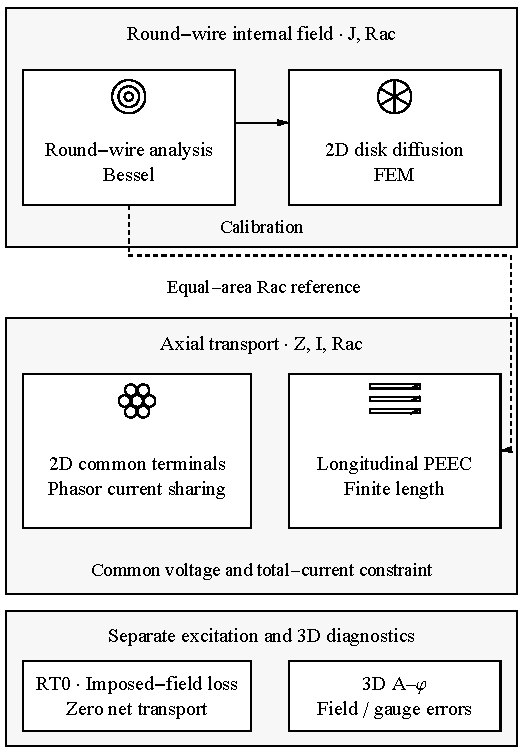
\includegraphics[width=\linewidth,height=.72\textheight,keepaspectratio]{../../assets/en/model_hierarchy.pdf}
\caption{Model hierarchy and comparable observables. Transport models are grouped by physical object and observable: round-wire internal fields support analytical and two-dimensional calibration, multistrand field–circuit models resolve common-terminal phasor currents, and longitudinal PEEC examines finite-length effects. Links identify internal-field calibration or equal-area resistance references. RT0 imposed-field loss and three-dimensional A–φ diagnostics occupy separate research scopes.}
\label{fig:model_hierarchy}
\end{figure}

% block-id: 01.automation.p1
\hypertarget{01.automation.p1}{}
Agent workflows connect source, Wolfram/Ansys MCP, bounded runners, and independent acceptance throughout the research. Six recorded case classes cover calibration, model construction and solution, cross-solver comparison, frequency extension, interface repair, and numerical failure diagnosis. This report connects the physical models to those execution records, showing how investigators can locate inputs, repeat calculations, and continue model development. \cite{CODEX,AGENTTOOLS,PYAEDTMCP}
